% Typografie a publikování
% 3. projekt
% Juraj Holub
% xholub40@stud.fit.vutbr.cz

\documentclass[a4paper, 11pt]{article}
\usepackage[utf8]{inputenc}
\usepackage[czech]{babel}
\usepackage[left=2cm,top=3cm,text={17cm,24cm}]{geometry}
\usepackage[IL2]{fontenc}
\usepackage[hyphens,spaces,obeyspaces]{url}
\usepackage{hyperref}
\usepackage[czech]{babel}
\usepackage{times}
\usepackage{dsfont}
\usepackage{multirow}
\usepackage{amsmath, amsthm, amsfonts, amssymb}
\usepackage[linesnumbered,noline,boxed,commentsnumbered,ruled,longend]{algorithm2e}
\SetNlSty{}{}{:} 
\usepackage{graphicx}
\usepackage{float}
\usepackage{lscape}
\usepackage{tikz}
\usepackage{lipsum}
\usepackage{tabularx,booktabs}

\newcolumntype{Y}{>{\centering\arraybackslash}X}

\author{Juraj Holub}
\date{}

\begin{document}


\begin{titlepage}
\begin{center}
	\Huge
	\textsc{\Huge{Vysoké učení technické v~Brně} \\
	\huge{ Fakulta informačních technologií}} \\
	\vspace{\stretch{0.382}}
	\LARGE{Formální jazyky a překladače} \\
	\Huge{Projektová dokumentácia} \\
	\Large{\today}
	\vspace{\stretch{0.618}}
	\setlength{\parindent}{0.3em}

	{\Large Tým 008, varianta II} \\
	
\begin{table}[H]
	\Large
	\centering
	\begin{tabular}{llc}
		\textbf{Člen}        & \textbf{Login} & \textbf{Rozdelenie bodov} \\
		Juraj Holub (vedúci) & \texttt{xholub40}       & 33\%                      \\
		Matej Parobek        & \texttt{xparob00}       & 33\%                      \\
		Samuel Krempský      & \texttt{xkremp02}      & 33\%                      \\
		Vitalina Koloda      & \texttt{xkolod02}       & 0\%                      
	\end{tabular}
\end{table}
		
\end{center}
\end{titlepage}

{\hypersetup{hidelinks}\tableofcontents}
\newpage

\section{Rozdelenie práce}

Prácu na projekte sme rozdelili následovne:
\begin{itemize}
	\item{\textbf{Lexikálnu analýzu} vytvoril Samuel Krempský (\texttt{xkremp02}).}
	\item{\textbf{Syntaktickú analýzu zhora nadol} vytvoril Matej Parobek (\texttt{xparob00}).}
	\item{\textbf{Precedenčnú syntaktickú analýzu} vytvoril Juraj Holub (\texttt{xholub40}).}
	\item{\textbf{Tabuľku symbolov} vytvoril Juraj Holub (\texttt{xholub40}).}
	\item{\textbf{Generátor výstupneho kódu} vytvoril Juraj Holub (\texttt{xholub40}) a Matej Parobek (\texttt{xparob00}).}
	\item{\textbf{Sémantickú analýzu} aplikovanú pri syntaktickej analýze zhora nadol vytvoril Matej Parobek (\texttt{xparob00}) a pre precedenčnú analýzu Juraj Holub (\texttt{xholub40}).}
\end{itemize}
\section{Lexikálna analýza}
Hlavnými funkciami Lexikálnej analýzy sú \texttt{get\_token()} a \texttt{ret\_token()}.   Funkcia \texttt{get\_token()} je implementovaná ako konečný automat. Vstup do tejto funkcie zaisťuje funkcia \texttt{getchar()}, ktorá číta znaky zo štandardného vstupu a Konečnému automatu sú predávané tieto znaky. Konečný automat e implementovaný pomocou podmienok využitia konštánt, ktoré sa nachádzajú v \texttt{enum states}. Ak sa Konečný automat dostane do konečného stavu tak vracia tzv. token.Niekedy však táto funkcia musí načítať aj jeden znak z ďalšieho tokenu, aby vedela,že je v konečnom stave.Tento znak je predávaný globálnou premennou \texttt{nextchar}. Token reprezentuje štruktúra majúca dva prvky \texttt{int type}, kde predávame typ daného tokenu pomocou konštánt a \texttt{string\_t attribute}, čo je premenná dátového typu \texttt{string\_t} pre prácu s dynamickými reťazcami, kde predávame názov premennej, alebo text dátového typu string v jazyku IFJ18. S takýmto vytovreným tokenom následne pracujú ďalšie časti prekladača.

Funkcia \texttt{ret\_token()} vracia token z parseru scanneru. Po tom, čo je táto funkcia spustená, tak pri ďalšom volaní je vrátený predošlý token. Táto funkcia je volaná parserom a môže požiadať až o dve predošlé tokeny, takže lexer musí mať stále uložené dva predošlé tokeny.

Ak scanner narazil na nesprávny znak, ktorý nie je povolený, je nesprávne zapísaný blokový komentár, alebo narazil na ostatné lexikálne chyby, tak parseru vracia token typu ERROR. Takýto spôsob riešenia chýb sme si vybrali kvôli správnemu uvoľňovaniu pamäte, aby sa správne najprv uvoľnila pamäť a až potom sa program ukončil.

Diagram konečného automatu, který specifikuje lexikální analyzátor \ref{fsm}.

\begin{figure*}[!]
	\centering
	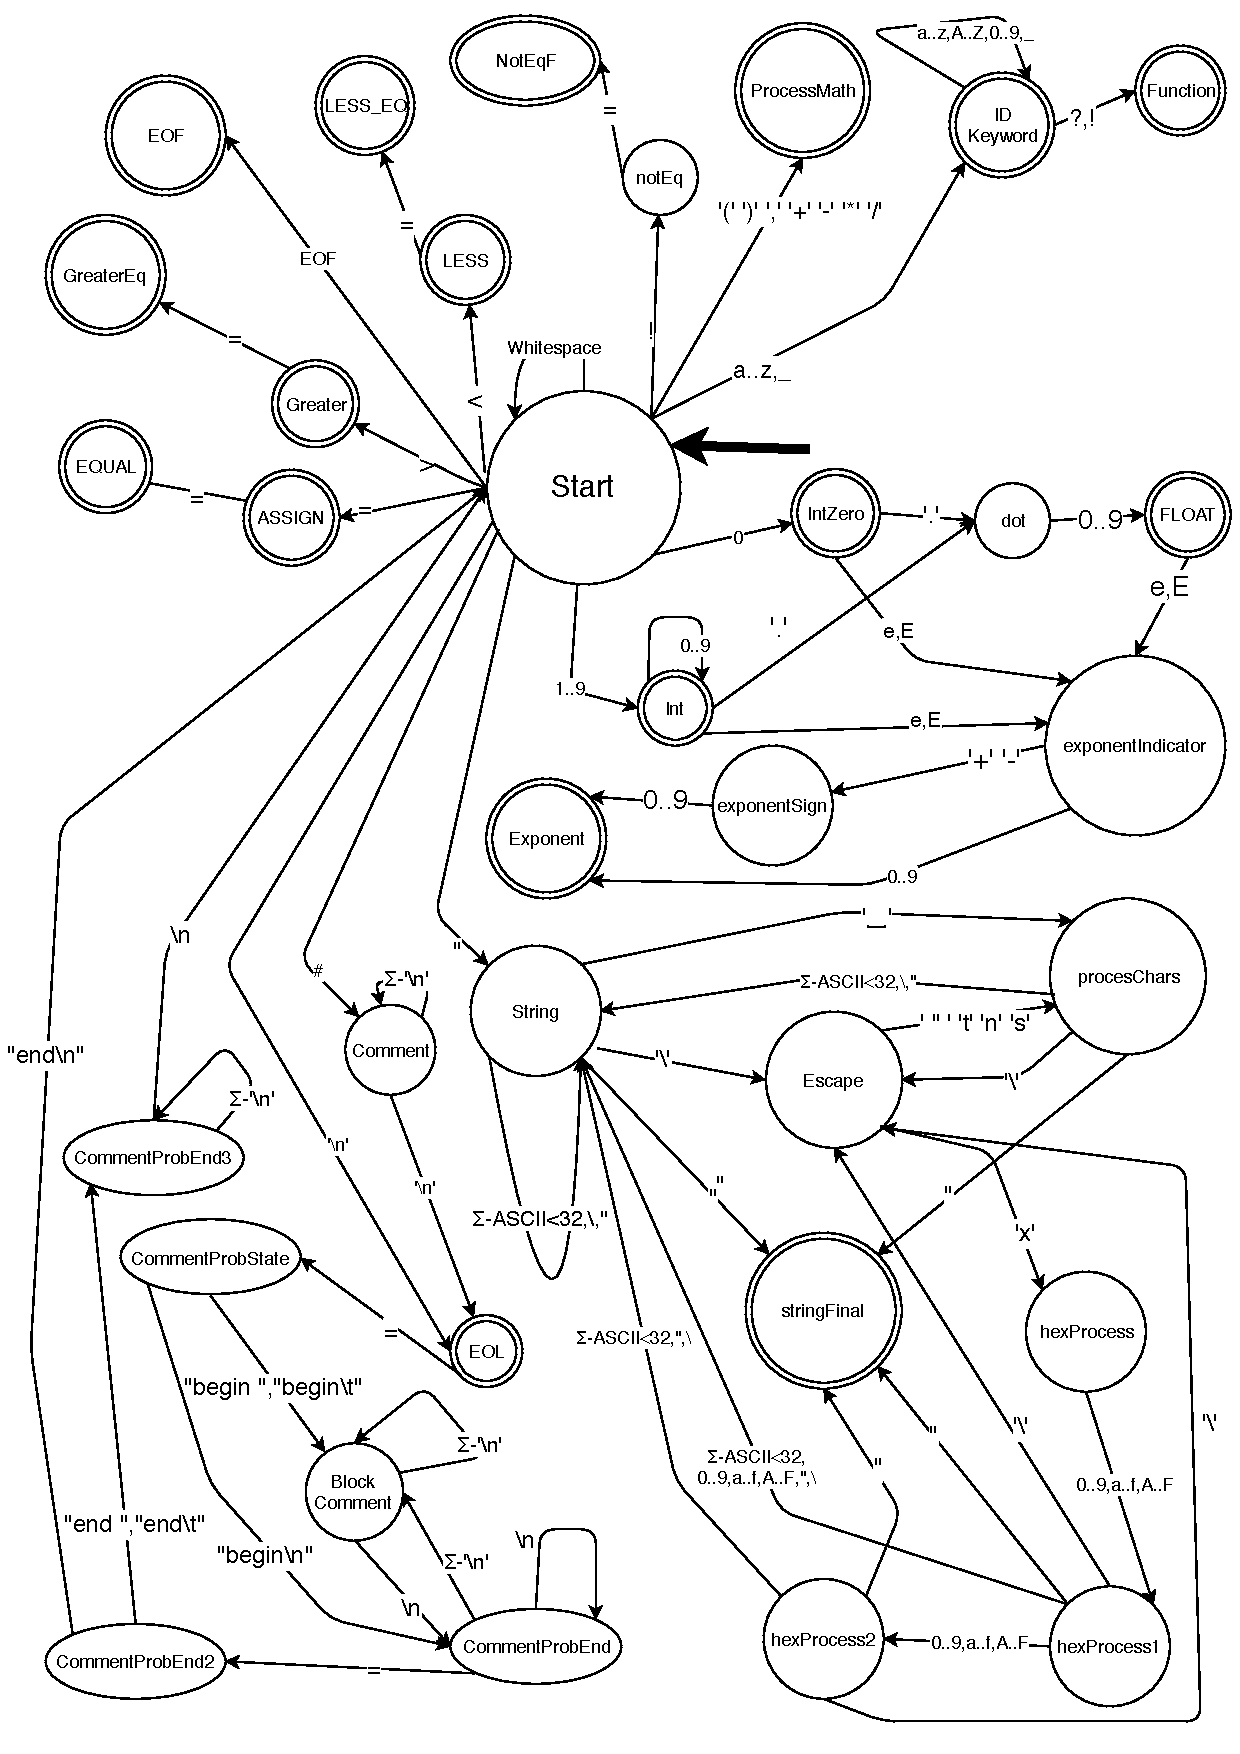
\includegraphics[width=\linewidth,height=8in]{fsm_scanner.pdf}\\[1pt]
	\caption{Diagram konečného automatu, který specifikuje lexikální analyzátor.}
	\label{fsm}
\end{figure*}


\section{Syntaktická analýza zhora nadol}
Matej
\section{Precedenčná syntaktická analýza}
Pre precedenčnú syntaktickú analýzu sme použili tabuľku \ref{prec_tab}. Symboly '$<$', '$>$', ' ' majú rovnaký význam ako značenie používané v predmete IFJ.
Legenda vstupných symbolov pre precedenčnú tabuľku \ref{prec_tab}:
\begin{itemize}
	\item{\textbf{NEG}: Operátor negácie boolovského výrazu (\texttt{\textbf{not}}) .}
	\item{\textbf{MINUS}: Operátor odčítania (\texttt{\textbf{-}}) typov float a integer.}
	\item{\textbf{PLUS}: Operátor sčítania alebo konkatenácia reťazcov (\texttt{\textbf{-}}).}
	\item{\textbf{MD}: Operátor násobenia alebo delenia (\texttt{\textbf{*}}, \texttt{\textbf{/}}).}
	\item{\textbf{EQ}: Relačný operátor (\texttt{\textbf{==}},\texttt{\textbf{!=}},\texttt{\textbf{<}},\texttt{\textbf{<=}},\texttt{\textbf{>}},\texttt{\textbf{>=}}).}
	\item{\textbf{ID}: Operand.}
	\item{\textbf{(}: Ľavá zátvorka vo výraze.}
	\item{\textbf{)}: Pravá zátvorka vo výraze.}
	\item{\textbf{\$}: Koniec výrazu (\texttt{\textbf{do}} , \texttt{\textbf{then}} , \texttt{\textbf{EOL}} , \texttt{\textbf{EOF}}) .}
\end{itemize}

\begin{table}[H]
	\centering
	\begin{tabularx}{\textwidth}{|c| *{9}{Y|}}%{|l|c|c|c|c|c|c|c|c|c|}
		\hline
		& \multicolumn{1}{c|}{\textbf{NEG}} & \multicolumn{1}{c|}{\textbf{MINUS}} & \multicolumn{1}{c|}{\textbf{PLUS}} & \multicolumn{1}{c|}{\textbf{MD}} & \multicolumn{1}{c|}{\textbf{EQ}} & \multicolumn{1}{c|}{\textbf{ID}} & \multicolumn{1}{c|}{\textbf{(}} & \multicolumn{1}{c|}{\textbf{)}} & \multicolumn{1}{c|}{\textbf{\$}} \\ \hline
		\textbf{NEG} & ' ' & ' ' & ' ' & ' ' & '\textless{}' & '\textless{}' & '\textless{}' & '\textgreater{}' & '\textgreater{}' \\ \hline
		\textbf{MINUS} & '\textgreater{}' & '\textgreater{}' & '\textgreater{}' & '\textless{}' & '\textgreater{}' & '\textless{}' & '\textless{}' & '\textgreater{}' & '\textgreater{}' \\ \hline
		\textbf{PLUS} & '\textgreater{}' & '\textgreater{}' & '\textgreater{}' & '\textless{}' & '\textgreater{}' & '\textless{}' & '\textless{}' & '\textgreater{}' & '\textgreater{}' \\ \hline
		\textbf{MD} & '\textgreater{}' & '\textgreater{}' & '\textgreater{}' & '\textgreater{}' & '\textgreater{}' & '\textless{}' & '\textless{}' & '\textgreater{}' & '\textgreater{}' \\ \hline
		\textbf{EQ} & '\textgreater{}' & '\textless{}' & '\textless{}' & '\textless{}' & '\textless{}' & '\textless{}' & \textbf{'\textless{}'} & \textbf{'\textgreater{}'} & \textbf{'\textgreater{}'} \\ \hline
		\textbf{ID} & '\textgreater{}' & '\textgreater{}' & '\textgreater{}' & '\textgreater{}' & '\textgreater{}' & ' ' & ' ' & '\textgreater{}' & '\textgreater{}' \\ \hline
		\textbf{(} & '\textless{}' & '\textless{}' & '\textless{}' & '\textless{}' & '\textless{}' & '\textless{}' & '\textless{}' & '=' & ' ' \\ \hline
		\textbf{)} & '\textgreater{}' & '\textgreater{}' & '\textgreater{}' & '\textgreater{}' & '\textgreater{}' & '\textgreater{}' & ' ' & '\textgreater{}' & '\textgreater{}' \\ \hline
		\textbf{\$} & '\textless{}' & '\textless{}' & '\textless{}' & '\textless{}' & '\textless{}' & '\textless{}' & '\textless{}' & '\textless{}' & ' ' \\ \hline
	\end{tabularx}
	\caption{Precedenčná tabuľka.}
	\label{prec_tab}
\end{table}

\section{Sémantická anylýza}
Juraj a Mato
\section{Generátor kódu}
Generovaný kód sme ukládali do listu, kde jedna položka listu predstavuje jednu inštrukciu v cieľovom jazyku IFJcode18. V liste sme aplikovali logické preusporiadanie vždy po ukončení vyhodnocovania aktuálneho rámca a to tak aby všetky premenné boli definované a inicializovane na hodnotu \texttt{nil} na začiatku daného rámca. Po ukončení všetkých analýz sme jedným priechodom vygenerovali celý list na štandartný výstup.
\section{Tabuľka symbolov}
Tabuľku symbolov sme implementovali ako \textbf{Tabuľku s rozptýlenými položkami} (\textbf{TRP}). Využili sme TRP s \textbf{explicitním} zreťazením synoným. TRP sme implementovali ako pole synoným o veľkosti 53 položiek. Veľkosť mapovacieho poľa sme zvolili ako prvočíslo a krok s veľkosťou jedna. Takúto veľkosť poľa synoným sme zvolili vzhľadom na jej výhodné chovanie, ktoré sme preberali v predmete IAL (nedochádza k vytváraniu zhlukov). Každá položka v mapovaciom poli obsahuje lineárny zoznam synoným. Keďže tabuľku využívame ako úložisko lexém programovacieho jazyka tak sme ako vyhľadávací kľúč použili názov identifikátoru premennej, ktorý musí byť unikátny. Pre vhodné mapovanie sme použili hashovaciu funkciu, ktorá poskytuje dobré výsledký pre reťazcové kľúče. Ako hash funkciu sme zvolili algoritmus \textbf{djb2}\footnote{Zdroj hash funkcie dbj2: 
	\urlstyle{rm}
	\url{http://www.cse.yorku.ca/~oz/hash.html}}
, ktorý má dobré výsledky práve pre reťazcové kľúče.
\section{Zhodnotenie}
Život je krásny.

%\begin{figure}[h]
%\centering
%\scalebox{0.4}\includegraphics{etiopan}
%\caption{Malý Etiopánek a jeho bratříček}
%	\label{obr1}
%\end{figure}


\end{document}
